\documentclass[%
reprint,nofootinbib,
amsmath,amssymb,
aps,
]{revtex4-1}
\usepackage{graphicx}% Include figure files
\usepackage{dcolumn}% Align table columns on decimal point
\usepackage{bm}% bold math
\usepackage[utf8]{inputenc}
\usepackage{listings}
\usepackage{amsmath}
\usepackage{physics}
\usepackage{booktabs}
\usepackage{float}
\usepackage[bottom]{footmisc}
\usepackage{scrextend}
\bgroup
\def\arraystretch{1.3}
\newcommand{\HRule}{\rule{\textwidth}{0.5mm}}
\makeatletter
\newcommand*{\rom}[1]{\expandafter\@slowromancap\romannumeral #1@}
\makeatother

\begin{document}
\onecolumngrid

\begin{center}
	\large\textbf{The Ising Model\\ \small{Studies of phase transitions in magnetic systems}}
\end{center}
\vspace{5mm}

\begin{center}
	\small{$^1$ Oline A. Ranum}\\
\end{center}

\begin{center}
	\small{$^1$ University of Oslo, Institute of physics, 
		olinear@student.matnat.uio.no}
\end{center}

\begin{center}
	\textit{\today}
\end{center}
\vspace{7mm}
\noindent 
\HRule \vspace{2mm}\\
The main objective of this paper is to 
\vspace{1.5mm}  \\
\HRule
\vspace{0.3cm}


\section{Introduction} \noindent 
\vspace{3mm}
\twocolumngrid
The Icing model was first developed
The Icing model describes
I first present theory

The Metropolis algorithm is based on the Markovian random walks and is widely applied in Monte Carlo simulations in the natural sciences. It is used in both studies of phase transitions in statistical physics and simulations of quantum mechanical systems.  

The Icing model has been extremely popular, with applications spanning from studies of phase transitions to simulations in statistics. 
 \newpage. \newpage 
\onecolumngrid
\section{Theory} \noindent 
\vspace{3mm}
\twocolumngrid
\subsection*{Thermodynamical systems} \noindent 
Finite, quantized systems with discrete properties will in general have a finite set of possible configurations $i$. When the temperature for such a system is sufficiently high and held constant it can be described using  Boltzmann statistics. I. e. the ensemble of microstates at any given temperature has the probability distribution \vspace{1mm}
\begin{equation}\label{tr}
P_i(\beta) = \dfrac{e^{-\beta E_i}}{Z}
\end{equation}  \vspace{1mm} \\ 
where $\beta^{-1} = k_bT$ and $k_b$ is the Boltzmann constant, T represents the temperature and $E_i$ the energy of a microstate $i$. It follows that the partition function for the canonical ensemble is given by\vspace{1mm}
\begin{equation}\label{pf}
Z = \sum_{i = 1}^{M}e^{-\beta E_i}
\end{equation}\vspace{1mm} \\ 
where M is the number of micro-states $i$ of the system. In general, such a system will have properties $X$ with moments \vspace{1mm}
\begin{equation*}
\expval{X^m} = \dfrac{1}{Z}\sum_iX_i^me^{-\beta E_i}
\end{equation*}\vspace{1mm} \\ 
For the expectation value of the energy, the following formula can also be derived \vspace{1mm} \\ 
\begin{equation}\label{ev}
\expval{E} = -\dfrac{\partial\ln Z}{\partial\beta}
\end{equation}\vspace{1mm} \\ 
It can furthermore be shown that the specific heat capacity $C_V$ of a system would be \vspace{1mm} \\ 
\begin{equation}\label{cv}
C_V = \dfrac{\beta}{T}\qty[\expval{E^2}-\expval{E}^2]
\end{equation}\vspace{1mm} \\ 
and susceptibility as a function of the magnetization $M$ \vspace{1mm} \\ 
\begin{equation}\label{chi}
\chi = \dfrac{\beta}{T}\qty[\expval{M^2}- \expval{M}^2] \vspace{4mm}
\end{equation} 
\hspace{6cm}[M. Jensen, 2015]

\subsection*{The Ising model} \noindent 
The Ising model is a ferromagnetic model consisting of discrete variables that represent magnetic dipole moments of atomic spin $s$. For a given critical temperature $T_c$, the Ising model exhibits a phase transition from a magnetic phase to a phase with zero magnetization. The model is a binary system where the objects at each lattice site can only take two values, for instance $s_\downarrow = -1$ and $s_\uparrow = 1$. In one or two dimensions the Ising model has analytical solutions to several expectation values and it gives a qualitatively good understanding of several types of phase transitions. \\ \indent 
In its simplest form the Ising model describes the energy of a configuration $i$ as  
\begin{equation}\label{isemodel}
	E = -J\sum_{\expval{kl}}^{N}s_ks_l -\mathcal{B} \sum_{k}^{N} s_k
\end{equation}
where $s_k = \pm 1$, N is the total number of spins and $J$ is a coupling constant expressing the strength of the interaction between neighboring spins. The formulation $\expval{kl}$ indicates the sum over nearest neighbors only. The parameter $\mathcal{B}$ is an external magnetic field interacting with the magnetic moment set up by the spins. The last contribution is omitted when there is no externally applied field.\\ \indent 
For a ferromagnetic ordering $J> 0$, meaning it is energetically favorable for neighboring spins to be aligned. It is a feature that leads to a cooperative phenomenon called spontaneous magnetization, for significantly low temperatures. In other words, through interactions between nearest neighbors, a given magnetic moment can influence the alignment of spins that are separated from the given spin by a macroscopic distance. The magnetization in such a system can be modeled as the sum over all spins for a given configuration $i$ as \\ 
\begin{equation}\label{mf}
M_i = \sum_{j = 1}^{N}s_j
\end{equation}
\hspace{6.9cm}[M. Jensen]
\subsection*{Periodic boundary conditions} \noindent 
For small systems, the way that the boundaries of the system are treated has an effect on the calculations. Periodic boundary conditions implies that the neighbor to the right of value $s_N$ is assumed to take the value of $s_1$, or equivalently that the neighbor to the left of $s_1$ takes the value $s_N$ [M. Jensen]. 


\subsection*{Ising model on 2x2 grid} \noindent 
For small systems, the boundary conditions matter. In the following it is assumed that the system is on a $2\times2$ lattice, with periodic boundary conditions. The arrangement of such a system is illustrated in figure \ref{si} in the appendix, where each individual spin $s_i$ can either be up or down. \\ \indent 
For a $2\times 2$ grid there exist $2^4 = 16$ different configurations. Various relevant properties of the $2\times 2$ system are presented below. The full derivations of the properties can be found in the appendix. The analytical partition function for this system is \\ 
\begin{equation} 
	Z =  4\cosh(8J\beta) + 12 
\end{equation} \\
The energy expectation values are \vspace{1mm} \\ 
\begin{align}\label{E}
	\expval{E} =& -\dfrac{32J}{z}\sinh(8J\beta) \\ &\nonumber\\
	\expval{E^2} =& \dfrac{258J^2}{Z}\cosh(8J\beta)
\end{align}\vspace{1mm} \\ 
It follows from equation \ref{cv} that \vspace{1mm} \\ 
\begin{align} \label{CV}
	C_V= \dfrac{\beta}{T}64J^2\qty[\dfrac{\cosh(8J\beta)}{\cosh(8J\beta) + 3}  -\qty(\dfrac{\sinh(8J\beta)}{\cosh(8J\beta) + 3 })^2]\nonumber  \\&\nonumber \\
\end{align}\vspace{1mm} \\ 
The magnetization expectation values becomes \vspace{1mm} \\ 
\begin{align} \label{exM}
	\expval{M} =&  0 \\ &\nonumber\\
\expval{\abs{M}} =&  \dfrac{2e^{8J\beta}}{\cosh(8J\beta) + 3 }\\ &\nonumber\\
\expval{M^2} =& \dfrac{8e^{8J\beta} + 8}{\cosh(8J\beta) + 3}
\end{align} \vspace{2mm}\\ 
Then, employing equation \ref{chi} the susceptibility becomes \vspace{1mm} \\ 
\begin{align}\label{CHI}
	\chi = \dfrac{\beta}{T}\dfrac{8e^{8J\beta} + 8}{\cosh(8J\beta) + 3}
\end{align}
\hspace{6.9cm}[M. Jensen]


\subsection*{Phase Transitions} \noindent 
It is the case that many physical quantities near the critical temperature $T_C$ can be described by a power law behavior. For instance, in the case of the Ising model the mean magnetization can be approximated as \\ 
\begin{equation}
\langle M(T) \rangle \sim \left(T-T_C\right)^{\beta}
\end{equation} \\ 
where $\beta=1/8$ is called the critical exponent. In a similar fashion, the heat capacity is approximated through \\ 
\begin{equation}
C_V(T) \sim \left|T_C-T\right|^{\alpha}
\end{equation} \\ 
with $\alpha = 0$, and the susceptibility \\
\begin{equation}
\chi(T) \sim \left|T_C-T\right|^{\gamma}
\end{equation} \\
with $\gamma = 7/4$. Such systems are furthermore characterized by the so-called correlation length, which is expected to be if th order if the grid spacing when  $T>> T_C$. The correlation length will increase as one approaches the critical temperature, due to the spins becoming more and more correlated as $T$ approaches $T_C$. One can describe the divergent behavior of the correlation length $\xi$ near $T_C$ as \\ 
\begin{equation}
\xi(T) \sim \left|T_C-T\right|^{-\nu}.
\label{eq:xi}
\end{equation}  \\ 
A correlation length that spans an entire system would characterize a second-order phase transition of that systems. For the case of numerical experiments one will always be limited to a finite grid, and therefore $\xi$ will only be proportional to the grid size. Through finite lattice scaling relations it is possible to relate the behavior at finite lattices with the results for an infinitely large lattice. The critical temperature then scales as \\
\begin{equation}
T_C(L)-T_C(L=\infty) = aL^{-1/\nu}
\label{eq:tc}
\end{equation}\\ 
with  $a$ a constant and  $\nu$ defined in Eq. (\ref{eq:xi}). By rearrangement of the terms one can express the thermodynamical critical temperature as 
\begin{equation}
	T_C(L=\infty) = T_C(L)-aL^{-1/\nu}
\end{equation}
Setting $\nu = 1$ we know after Lars Onsager that the exact result for the critical temperature is
\begin{equation}
	\dfrac{k_bT_C}{J} = \dfrac{2}{\ln(1+\sqrt{2})} \approx 2.269
\end{equation}
Thus, the critical temperature of two final grids can be used to estimate the constant $a$ as \\ 
\begin{equation}
	a = \dfrac{T_C(N_1)-T_C(N_2)}{N_1^{-1/\nu}-N_2^{-1/\nu}}
\end{equation}


\subsection*{Monte Carlo Markov Chains} \noindent 
The Monte Carlo simulations are excellent tools to simulate statistical systems. A Markov procedure is in its essence a random walk to yield new configurations of a selected system. The random walk is set with a chosen probability for making a transition, such that the new configuration is independent of the previous history of the system. Markov Chains are today employed in Monte Carlo schemes to generate new random states, with the reasoning that by iteratively employing such a random selection the system will over time converge to its most likely state. In thermodynamics, this is means that the system will converge towards an equilibrium distribution and the numerical system will mimic the way a real system reaches its most likely state. In order to reach this distribution, the Markov process obeys conditions of ergodicity and detailed balance imposing constraints on accepting or rejecting new random states. \\ \indent 
The Markov Chain theory builds on an evolution of a probability distribution function (PDF), where for a given transition probability $W(j\rightarrow i)$ the PDF $w_i$ at a time $t+ \epsilon$ is related to $w_i$ at time $t$ through the stochastic matrix $\sum_j W_{ij} = 1$ of the Markov chain equation \\ 
\begin{equation}\label{MCE}
	w_i(t+ \epsilon) = \sum_j W_{ij}w_j(t) = \sum_j W(j\rightarrow i)w_j(t)
\end{equation} \\ 
I.e. a representation of the discretized time-development of an original PDF. Both $W$ and $w$ represent probabilities and are subjected to the constraint that for every $t$ \\ 
\begin{equation*}
	\sum_i w_i(t) = 1 \textnormal{ \& } \sum_j W(j\rightarrow i) = 1
\end{equation*}
\hspace{6.9cm}[M. Jensen] \\
\vspace{6mm}

\subsection*{The Metropolis algorithm} \noindent 
The Metropolis algorithm is one of the most used algorithms for generating new configurations based on Markovian random walks. In most situations, the transition probability $W_{ij}$ is unknown, but it can be modeled using the Metropolis algorithm by splitting the probability expression in two parts \\ 
\begin{equation}\label{MCE2}
	W(i\rightarrow i) = T(j\rightarrow i)A(j\rightarrow i)
\end{equation} \\ 
where $T(j\rightarrow i)$ is the likelihood for having a transition and $A(j\rightarrow i)$ is the likelihood for accepting a suggested transition. \\
The Metropolis algorithm can then be expressed in two parts. Initially, a transition is proposed to a new configuration $i$ with a transition probability $T(j\rightarrow i)$. Then, the transition is accepted or rejected based respectively on an acceptance probability $A(j \rightarrow i)$ or denial probability $1-A(j \rightarrow i)$. If accepted, the configuration $i$ is employed as the new initial condition for the next transition. From this procedure the dynamical process towards equilibrium can be derived. Equation \ref{MCE} can be rewritten using equation \ref{MCE2} as \\ 
\begin{align}
	w_i(t+\epsilon) =& \sum_j W_{ij}w_j(t) \nonumber\\ =& \sum_j [T(j\rightarrow i)A(j\rightarrow i)w_j(t) \nonumber\\&+ T(j\rightarrow i)(1-A(j\rightarrow i))]
\end{align} \\ 
with the condition that $\sum_j T(j\rightarrow i) = 1$, one gets that \\ 
\begin{align}
w_i(t+\epsilon) - w_i(t) =& \sum_j W_{ij}w_j(t)  \nonumber\\ =  & \sum_j [T(j\rightarrow i)A(j\rightarrow i)w_j(t) \nonumber \\ &+ T(i\rightarrow j)A(i\rightarrow j)w_i(t)]
\end{align} \\ 
This implies that in the limit of $t\rightarrow \infty$, then $w_i(t) \rightarrow w_i$ and \\
\begin{equation}
	w_i(t+\epsilon) = w_i(t)
\end{equation}\\ 
From this, we can employ the concept of detailed balance to deduce the transition probability, where detailed balance can be expressed as \\
\begin{equation}
	W(i\rightarrow j)w_i = W(j \rightarrow i)w_j
\end{equation} \\
Elaborating on equation \ref{MCE2} in the equilibrium condition \\ 
\begin{align}\label{probe}
	0 &=  \sum_j W_{ij}w_j(t) \nonumber \\ &= \sum_j [T(j\rightarrow i)A(j\rightarrow i)w_j(t) + T(i\rightarrow j)A(i\rightarrow j)] \nonumber\\
	& \nonumber\\
	\implies & T(j\rightarrow i)A(j\rightarrow i)w_j(t)\nonumber \\  &= T(i\rightarrow j)A(i\rightarrow j)w_i(t)\nonumber \\ 
	& \nonumber\\
	\implies& \dfrac{w_i}{w_j} = \dfrac{T(j\rightarrow i)A(j\rightarrow i)}{T(i\rightarrow j)A(i\rightarrow j)}
\end{align} \\ 
Employing ergodicity, the hypothesis which states that in equilibrium all available
states of a closed system have equal probability, $T(j\rightarrow i) = T(i \rightarrow j)$ then \\
\begin{equation}
	\dfrac{w_i}{w_j} = \dfrac{A(j\rightarrow i)}{A(i\rightarrow j)}
\end{equation} \\ 
From equation \ref{tr} it is known that \\
\begin{equation}
	w_i \rightarrow P_i(\beta) = \dfrac{e^{-\beta E_i}}{z}
\end{equation} \\ 
Inserting this back into equation \ref{probe}, 
so that the transition rate can be expressed as \\
\begin{align} \label{probrate}
	\mathcal{P} =  \dfrac{P_i}{P_j} = \dfrac{w_i}{w_j} &  = \dfrac{A(j\rightarrow i)}{A(i\rightarrow j)}  = \dfrac{\dfrac{e^{-\beta E_i}}{z}}{\dfrac{e^{-\beta E_j}}{z}} \nonumber \\ & \nonumber \\ 
     \implies \mathcal{P} & =  e^{-\beta \Delta E}
\end{align} \\ 
where $\Delta E = E_i - E_j$.

\subsection*{Probability distribution functions}\noindent
For a broad range of Monte Carlo applications, the only requirement is that a probability distribution function (PDF) that describes the physical system is known. Once a PDF is established a Monte Carlo simulation can proceed by taking random samplings from the PDF. The result is built on the average of many simulations over the number of observations, so the variance can be predicted. The PDF is a function $p(x)$ on the domain which in the discrete case gives us the probability or relative frequency with which these values of X occur \vspace{0.5mm} \\
\begin{equation*}
p(x) = \textnormal{Prob}(X=x)
\end{equation*}\vspace{0.5mm} \\
The PDF must satisfy two properties. First, the PDF has to be normalized so that all the probabilities add up to unity\vspace{0.5mm} \\
\begin{equation*}
\sum_{x_i\in \mathcal{D}} p(x_i) = 1
\end{equation*} \vspace{0.5mm} \\
Secondly, assuming that the PDF is normalized, the probability has to be of a positive nature \vspace{0.5mm} \\
\begin{equation*}
0 \leq p(x) \leq 1
\end{equation*}\vspace{0.5mm} \\
One especially important PDF is the uniform distribution\vspace{2mm} \\
\begin{equation}\label{unipdf}
p(x) = \dfrac{1}{b-a}\Theta(x-a)\Theta(b-x)
\end{equation}\vspace{0.5mm} \\
where 
\begin{align}
\Theta(x) &= 0& \hspace{2mm} x < 0 \nonumber \\
\Theta(x) &= 1& \hspace{2mm} x \geq 0 
\end{align}\\ 
\subsection*{Error Analysis}
\noindent 
The variance of a stochastic variable X is defined as\\
\begin{align}\label{var}
\textnormal{VAR}(x) = \sigma_X^2 &= \expval{(x-\expval{x})^2} \nonumber \\
&= \int(x-\expval{x})^2p(x)dx\nonumber\\
&= \int(x^2-2x\expval{x}^2+ \expval{x}^2)p(x)dx\nonumber\\
& = \expval{x^2} - \expval{x}^2 \nonumber \\ 
\end{align} \\
\hspace{6cm}[Press et al.]  \\ 
The standard deviation is then provided as \\ 
\begin{align}\label{std}
	\textnormal{STD}(x) = \sigma_X &= \sqrt{\expval{x^2} - \expval{x}^2 \nonumber } 
\end{align} 


\onecolumngrid
\newpage 
\section{Method} \noindent 
\twocolumngrid 
\noindent 
\subsection*{General system setup} \noindent 
A square lattice $S$ consisting of $L\times L$ grid-points are initiated, and filled with spin values $s_i = \pm 1$.  The square lattice is initiated in two separate ways, one of a ordered structure with all grid-points containing spin up and one of a random structure where the grid-points are filled at random with spin up or spin down using a Mersenne Twister 19937 random number generator. \\ 
\indent The initial energy of the system is evaluated using the Ising model of equation \ref{isemodel} with $J = 1$, and the initial magnetization using equation \ref{mf}. In order to propagate the state of the system towards its equilibrium state a Monte Carlo Metropolis approach with periodic boundary conditions is employed in the following manner: \\ 
\indent Two random indices $i$ and $j$ are drawn using the Mersenne Twister 19937 random number generator with a uniform integer distribution ranging from 0 to $L$. The indices are employed to select the matrix element $S_{ij}$, whose spin value is flipped. The energy from preforming the spin flip is calculated. If the change of spin orientation of spin $S_{ij}$ yields a lower energy or energy change of 0, the transition to the configuration with the flipped spin of $S_{ij}$ is preformed. If the transition would yield a higher energy, a random real number is drawn from a normal distribution of numbers $i\in[0,1]$ by the Mersenne Twister. If the random number is lower than the probability rate of equation \ref{probrate}, the transition is also made. When a transition is preformed, the energy and magnetization of the system is reevaluated in accordance to equation \ref{isemodel} and \ref{mf}. In all other cases, the transition is rejected and the initial configuration and properties of the system are conserved. This procedure is run N times, representing the number of Monte Carlo iterations.\\ \indent
\subsection*{2$\times$ 2 grid evaluation} \noindent 
The number of grid points $L^2$, the number of Monte Carlo Cycles $N$ and the set temperature $T$ is read from text files. Initially, a grid consisting of $2\times 2$ spins are considered for a randomly initiated $S$-matrix. The systems analytical expectation values and properties are calculated using equation \ref{E}-\ref{CHI}. These calculations are used as benchmark values for the following numerical estimates, and are presented in table \ref{bc}. The system is then evaluated using the above procedures, setting $T = 1.0$ $k_bT/J$  and $N = 10^n$ with $n \in [4,5,6,7,8]$. \\ \indent 
 From the energy and magnetization values the expectation values of $E$, $E^2$, $M$, $M^2$ and $\abs{M}$ are calculated by summing over all simulated values of $E$ and $M$ weighted by the number of Monte Carlo Cycles. An initial burn-in time is set at $t_{burn} = 5\times10^{-3}N$. Then $C_V$ and $\chi$ is estimated using equation  \ref{cv} and \ref{chi}. The expectation values and properties are weighted with the number of spins in the system, to yield the property values per spin. This procedure is preformed 10 times, and the final results are presented as the average of all runs. The results are presented in table \ref{bc} and compared to the benchmark values of the analytical predictions. 
\subsection*{20$\times$20 grid evaluation and analysis of most likely states} \noindent 
The grid size is increased to $20\times20$, and the procedure is repeated for both the randomly initiated and ordered matrix $S$. Using the number of Monte Carlo iterations as an evolution axis, the expectation values are estimated as a function of $N$. The evaluation is preformed for both $\expval{E}$ and $\expval{\abs{M}}$ for both  $T = 1.0$ $k_bT/J$ and $T = 2.4$ $k_bT/J$. The number of accepted iterations as a function of $N$ is also plotted for both temperatures. The result is presented as the mean of 10 independent runs, and provided with the variance as error bars. An estimate for the equilibration time is provided based on a graphical evaluation. 
\subsection*{Analysis of the probability distribution} \noindent
The probability distribution $P(E)$ is estimated by counting up the numbers of times a given energy appears in the computations, for both temperatures. The burn-in time is now set to $t_{burn} = 5000L^2$. The results are presented using the \textit{seaborn kde-based distplot} histograms. The results are compared with the computed variance in energy $\sigma_E^2$ as given by equation \ref{var}. 
\subsection{Numerical studies of phase transitions} \noindent 
In order to study the behavior of the Ising model close to the critical temperature, $\expval{E}$, $\expval{\abs{M}}$, $C_V$ and $\chi$ are evaluated as functions of temperature. The properties are calculated for $T\in[2.15,2.5]$ $k_bT/J$ with step interval $dT = 10^{-3}$ $k_bT/J$ for $L\in[40, 60, 80, 100]$. The result are compared to the analytical value of $T_c$ as derived by L. Onsager. 
 
\subsection{Parallelization}\noindent 
The implementation is parallelized using MPI on four processors. An analysis of the time is preformed using various optimization flags. \\
 
\newpage 
\onecolumngrid
\section{Results} 
\begin{figure}[H] 
	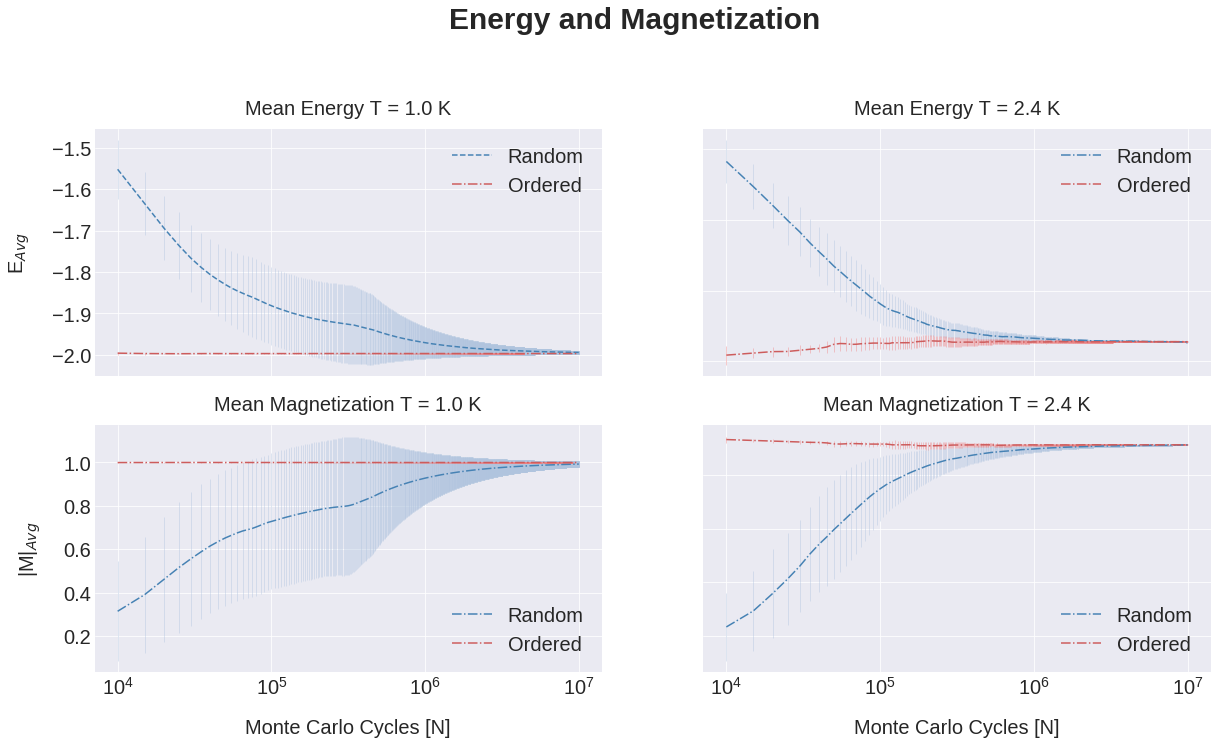
\includegraphics[width = \textwidth]{Figures/4C1.png} 
	\caption{\label{4C11}The energy- and absolute magnetization expectation value per spin, as function of Monte Carlo iterations $N$. Each point is the sum of the previous $N_i$ points averaged by $N_i$. The error bars represents the standard deviation of the 10 independent test runs. \vspace{11mm}}
\end{figure}
\twocolumngrid
\subsection*{2$\times$2 Ising Model}\noindent 
The predicted property values of a $2\times 2$ lattice is presented in table \ref{2b}, alongside the analytical predictions on the estimations. It is evident that the properties exhibit various precision for a selected $N$ in regards to the analytical predictions. While $\expval{E}$, $\expval{M^2}$ and $\chi$ converges to a precision of four digits at $N=10^7$, while $C_V$ reaches a precision of three leading digits. $\expval{E^2}$, $\expval{\abs{M}}$ and  $\expval{M} $ reach the poorest precisions at respectively 0 and 2 leading digits for the two latter. It appears that $N=10^7$ is sufficient to make a decent approximation to the analytical values. \\ \indent 
The results of the Monte Carlo Metropolis approach to estimating $\expval{E}$ and $\expval{\abs{M}}$ are plotted in figure \ref{4C11}, as functions of the number of Monte Carlo iterations. For both temperatures it is evident that the system who was initiated in the ground state exhibit evaluations more consistent with the analytical predictions for low $N$. The system initiated at a random state has a longer equi-\\ \vspace{10mm} 
\begin{table}[H]
	\caption{\label{2b}Results per spin of a Metropolis Algorithm using the Ising model on a $2\times 2$ spin-grid. The results are provided as functions of N, for $T = 1.0$ $k_bT/J$. The analytical expectation values are given at the bottom of the table as A.}
	\begin{tabular}{|c|c|c|c|c|c|c|c|} \hline 
		\textbf{N}  & \hspace{1mm}	$\expval{\mathbf{E}}$ \hspace{1mm} & \hspace{1mm}$\expval{\mathbf{E^2}}$ \hspace{1mm} & \hspace{1mm}	$\expval{\mathbf{M}}$\hspace{1mm}  &	\hspace{1mm} $\expval{\mathbf{M^2}}$ \hspace{1mm}  &	\hspace{1mm}$\expval{\abs{\mathbf{M}}} $\hspace{1mm} & \hspace{2mm}$\mathbf{\chi}$	\hspace{2mm} & \hspace{2mm}	\textbf{C}$_V$\hspace{2mm} \\ \hline 
		&&&&&&&\\
		10$^4$   &  -1.9974   & 15.9793  &  0.6353 &   3.9958 &   0.9992&   0.0207 &   1.7822\\
		10$^5$    &          -1.9967   & 15.9739  &  -0.0309 &   3.9946 &   0.9989&   0.0260 &   3.7958\\ 
		
		10$^6$  &          -1.9958   & 15.9667  &  -0.0351 &   3.9931 &   0.9986&   0.0332 &   3.9452\\ 
		
		10$^7$  &          -1.9960   & 15.9680  &  -0.0037 &   3.9933 &   0.9987&   0.0320 &   3.9897\\ 
		10$^8$   &          -1.9960   & 15.9678  &  -0.0015 &   3.9933 &   0.9987&   0.0321 &   3.9931\\ 
		&&&&&&&\\ \hline 
		A &-1.9960 & 16.0926  &0.    &  3.9933 & 0.9980  & 0.0321&  3.9933 \\ \hline 
	\end{tabular}
\end{table} \newpage 
\begin{figure}[H]
	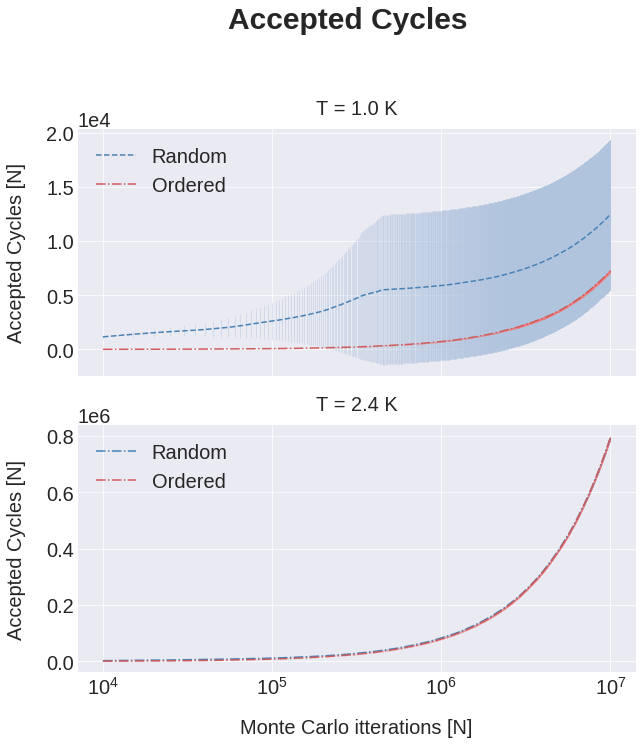
\includegraphics[width = \columnwidth]{Figures/Plot2.png} 
	\caption{\label{4C2}The number of accepted transitions in the spin configuration as a function of N Monte Carlo iterations for configurations initiated in both an orderly and random fashion. The errobar represents the variance of 10 independent runs. \vspace{10mm}
	}
\end{figure} 

\begin{figure}[H]
	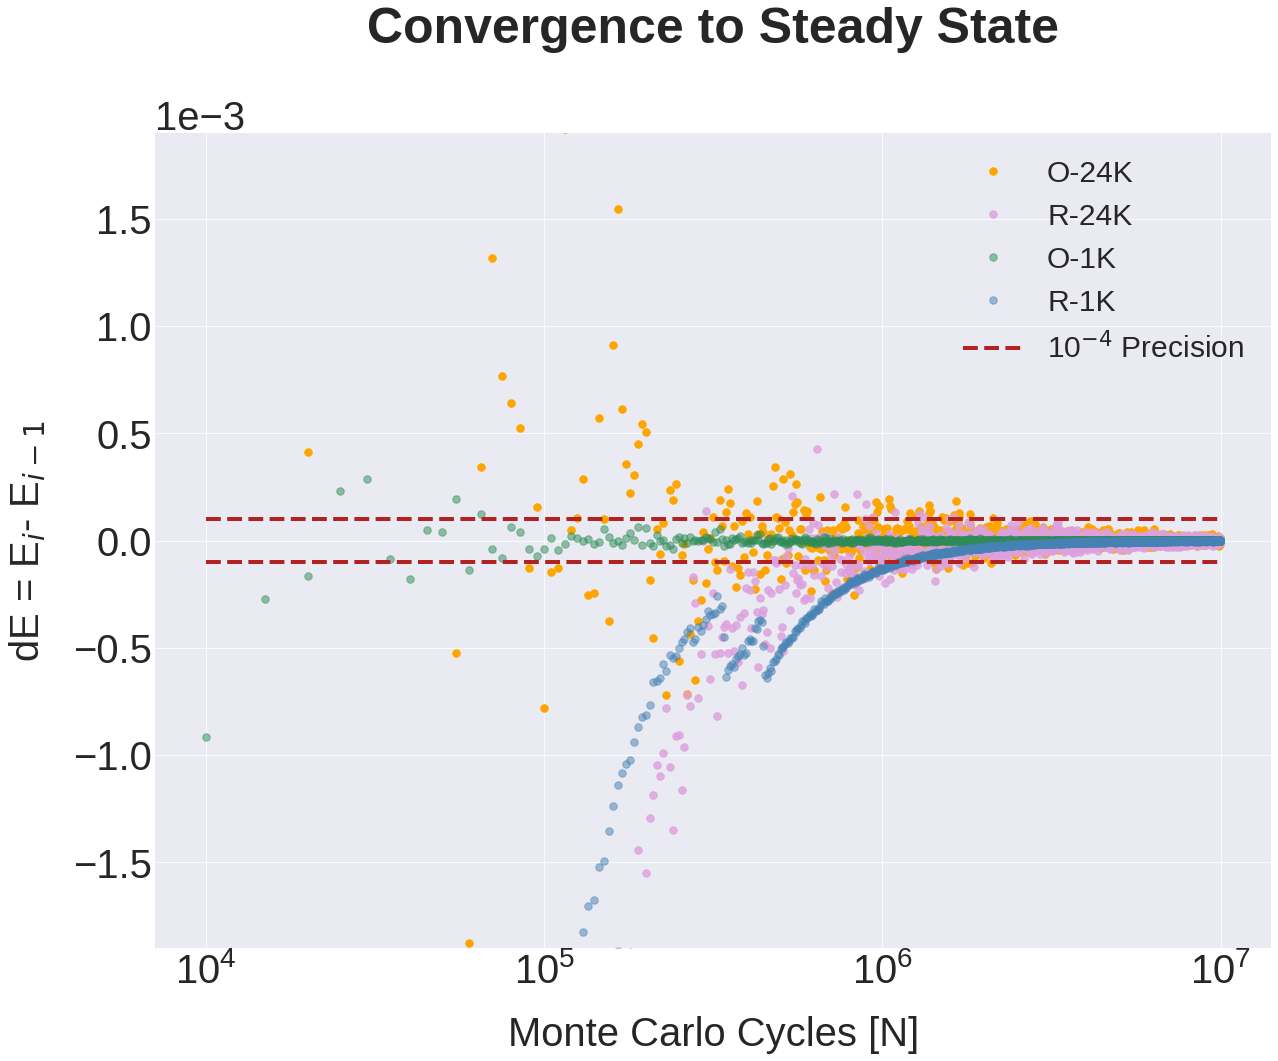
\includegraphics[width = \columnwidth]{Figures/Plot3.png} 
	\caption{\label{4C3} The energy difference between two Monte Carlo iterations as function of N. Data is shown for the temperatures $T = 1.0$ $k_bT/J$ and $T = 2.4$ $k_bT/J$, for both random and ordered initial states $S$. The threshold indicated by the red strips is a precision of $10^{-4}$ digits.}
\end{figure}  \newpage 

\noindent libration time. The equilibration time appears to be a bit smaller for $T = 2.4$ $k_bT/J$ than it is for $T = 1.0$ $k_bT/J$, although both initial $S$ matrices for both temperatures appears to have converged by the time $N = 10^7$. \\ \indent 
It is furthermore evident in figure \ref{4C11} that the curves converge towards $\expval{E} = -1.996$ and the magnetization to $\expval{\abs{M}} = 0.998$. A graphical evaluation of figure \ref{4C11} that the equilibration time for $T = 1.0$ $k_bT/J$ is roughly \\
\begin{equation*}
	t_{eq} \approx 10^7 \hspace{3mm}[N]
\end{equation*}\\
 while for $T = 2.4$ $k_bT/J$ the equilibration time is roughly \\  
 \begin{equation*}
 t_{eq} \approx 10^6 \hspace{3mm}[N]
 \end{equation*} \\ 
The variance of the system initiated with the random initial spin configuration of $S$, while the $S$ matrix initiated with an ordered spin configuration has barely a visible variance. In both cases the variance goes to zero for sufficiently large $N$-values. \\ 
Figure \ref{4C2} shows the number of accepted cycles as a function of the number of Monte Carlo iterations $N$. It is evident that the difference in number of accepted cycles following an ordered or random initial state are larger for $T = 1.0$ $k_bT/J$ than it is for $T = 2.4$ $k_bT/J$. It is furthermore clear that the number of accepted cycles grows larger more rapidly for $T = 2.4$ $k_bT/J$. \\ \indent  
Figure \ref{4C3} shows the change in energy for each new configuration $i$, $dE = E_i-E{i-1}$. Here, it becomes evident that the $dE$ become constant equal to zero as $N$ increases, and the equilibrium state is reached. The spread in $dE$ is fluctuating more in the case where the evaluation was initiated using a random state, that it was using an ordered state. As well, again it is evident that the ordered state has a lower equilibration time than the random initial state. \\ \indent 
Figure \ref{4C4} shows the energy distribution as a function of T. For $T = 1.0$ $k_bT/J$ one can observe two primer bins. The largest selection of $E$ values are found at $E = -800$, while a somewhat smaller fraction is found at $E = - 792$. For $T = 2.4$ $k_bT/J$ it is evidently a broad range of distributed energies present, with a mean of $E = -700$. The curve enveloping the bins are the fitted curve. 

\newpage 

\onecolumngrid

\begin{figure}[H]
	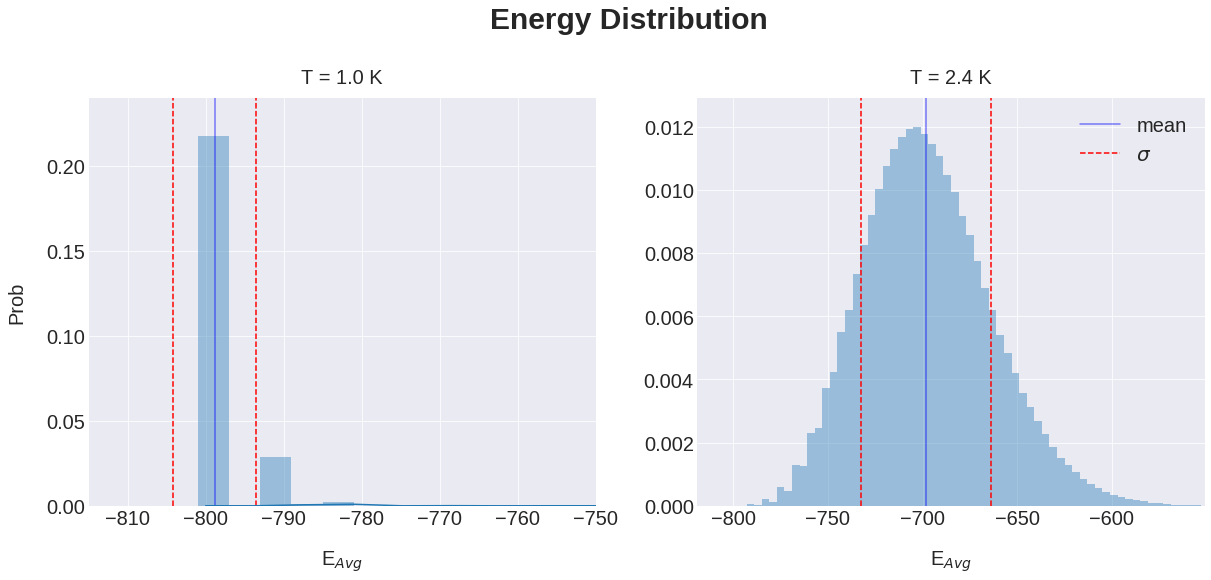
\includegraphics[width = \textwidth]{Figures/Plot4E.png} 
	\caption{\centering \label{4C4} \vspace{29mm}}
\end{figure} 

\twocolumngrid

\newpage.
\newpage.
\newpage.
\section{Discussion} \noindent 
\section{Conclusion} \noindent 
\newpage . \newpage
\onecolumngrid 
\section{References} \noindent
\newpage
\section{Appendix} \noindent
\subsection{Derivation of thermo-physical quantities for a $2\times 2$ lattice grid}
\begin{figure}
	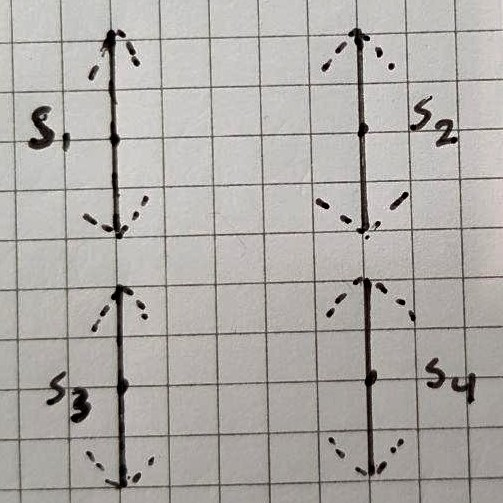
\includegraphics[scale = 0.5]{Figures/si.jpg}
	\caption{\label{si}}
\end{figure}
Each energy state for the various configurations are determined by equation \ref{isemodel}, who for the specific $2\times2$ lattice grid is
\begin{align*}
E_i  =& -J[s_1s_2 + s_1s_3 + s_2s_1+s_2s_4+s_4s_2+s_4s_3 + s_3s_1 + s_3s_4] \nonumber \\
= &-2J[s_1s_2 + s_2s_3 + s_3s_4 + s_4s_1]
\end{align*}\vspace{1mm} 
One can use this relation to estimate the analytical partition function \footnote{By identity: $2\cosh(\alpha) = e^{-\alpha} + e^{\alpha}$}
\begin{align*}
Z = \sum_{i = 1}^{16}e^{2J\beta[s_1s_2 + s_2s_3 + s_3s_4 + s_4s_1]}
=&  2e^{-8J\beta} + 2e^{8J\beta} + 12e^0\nonumber \\
= & 4\cosh(8J\beta) + 12 
\end{align*} 
Using equation \ref{ev} it is evident that the energy expectation value for the system becomes 
\begin{align*}
\expval{E} = -\dfrac{\partial ln Z}{\partial \beta} = -2\dfrac{\partial}{\partial \beta}\ln{[e^{-8J\beta} + e^{8J\beta}]} =& -\dfrac{16J}{Z}[e^{8J\beta} - e^{-8J\beta}] \\ 
& = -\dfrac{32J}{z}\sinh(8J\beta)
\end{align*}
Table \ref{bc} shows all configurations and their corresponding energy $E_i$ and magnetization $M_i$

\begin{table}[!h]
	\caption{\label{bc} The 16 configurations for a $2\times 2$ Ising model on a 2D lattice. The energy $E_i$ and magnetization $M_i$ for each configuration $i$ is provided.}
	\begin{tabular}{|c|c|c|c|} \hline 
		S$_i$&S$_\uparrow$ & \textbf{$E_i$} [J]&$ M_i$ [\#] \\ \hline   
		0& $\uparrow\uparrow\uparrow\uparrow$ &-8J&4\\
		1&$\uparrow\uparrow\uparrow\downarrow$ & 0&2\\
		2&$\uparrow\uparrow\downarrow\uparrow$ &0&2\\
		3&$\uparrow\downarrow\uparrow\uparrow$ &0&2\\
		4&$\downarrow\uparrow\uparrow\uparrow$ &0&2\\
		5&$\uparrow\uparrow\downarrow\downarrow$ &0&0\\
		6&$\downarrow\downarrow\uparrow\uparrow$ &0&0\\
		7&$\uparrow\downarrow\uparrow\downarrow$ &0&0\\
		8&$\downarrow\uparrow\downarrow\uparrow$ &0&0\\
		9&$\downarrow\uparrow\uparrow\downarrow$ &8J&0\\
		10&$\uparrow\downarrow\downarrow\uparrow$ &8J&0\\
		11&$\uparrow\downarrow\downarrow\downarrow$ &0&-2\\
		12&$\downarrow\uparrow\downarrow\downarrow$ &0&-2\\
		13&$\downarrow\downarrow\uparrow\downarrow$ &0&-2\\
		14&$\downarrow\downarrow\downarrow\uparrow$ &0&-2\\
		15&$\downarrow\downarrow\downarrow\downarrow$ &-8J&-4\\\hline 
	\end{tabular}
\end{table}


The specific heat capacity of this system can be calculated using equation $cv$, 
\begin{align}
\expval{E^2} = \dfrac{1}{Z}\sum_{i=1}^{16}E_ie^{-\beta E_i}  = & \dfrac{128J^2}{Z}(e^{8J\beta} + e^{-8J\beta}) \\
=& \dfrac{258J^2}{Z}\cosh(8J\beta)
\end{align}
It follows that 
\begin{align}
C_V =& \dfrac{\beta}{T}\qty[\dfrac{258J^2\cosh(8J\beta)}{4\cosh(8J\beta) + 12 }  -\qty(-\dfrac{32J\sinh(8J\beta)}{4\cosh(8J\beta) + 12 })^2] \nonumber \\
= & \dfrac{\beta}{T}64J^2\qty[\dfrac{\cosh(8J\beta)}{\cosh(8J\beta) + 3}  -\qty(\dfrac{\sinh(8J\beta)}{\cosh(8J\beta) + 3 })^2]\nonumber \\ \nonumber & \\ & 
\end{align}
The mean magnetization becomes 
\begin{align*}
\expval{M} =& \dfrac{1}{Z}\sum_{i = 1}^{16} M_ie^{-\beta E_i} \\ 
= & \dfrac{1}{Z}\qty(4e^{8J\beta} +4\times 2e^0 + 4\times(-2)e^0 -4e^{8J\beta}) \\
= & 0
\end{align*}
\begin{align*}
\expval{\abs{M}} =& \dfrac{1}{Z}\sum_{i = 1}^{16} \abs{M_i}e^{-\beta E_i} \\ 
= & \dfrac{1}{Z}\qty(4e^{8J\beta} +4\times 2e^0 + 4\times2e^0 +4e^{8J\beta}) \\
= & \dfrac{8e^{8J\beta}}{4\cosh(8J\beta) + 12 } \\
= & \dfrac{2e^{8J\beta}}{\cosh(8J\beta) + 3 }
\end{align*}
\begin{align*}
\expval{M^2} =& \dfrac{1}{Z}\sum_{i = 1}^{16} M_i^2e^{-\beta E_i} \\ 
= & \dfrac{1}{Z}\qty(16e^{8J\beta} +4\times 4e^0 + 4\times4e^0 + 16e^{8J\beta}) \\
= & \dfrac{8e^{8J\beta} + 8}{\cosh(8J\beta) + 3}
\end{align*}
Yielding the susceptibility 
\begin{align}
\chi =& \dfrac{\beta}{T}\qty(\expval{M^2}- \expval{M}^2)\\
=& \dfrac{\beta}{T}\dfrac{8e^{8J\beta} + 8}{\cosh(8J\beta) + 3}
\end{align}

 
\end{document}